\chapter{Requisitos do Sistema}

\chapter{Arquitetura da Aplicação}


\section{Modelo de Dominio }
Todo e qualquer projeto possui um domínio específico. O modelo de domínio deve capturar os seguintes pontos: as entidades, os relacionamentos entre as entidades e o vocabulário de domínio do problema. Para além disso também deve ser uma visão estática do problema onde é possível representar as regras de negócio invariantes no tempo. Ou seja, o modelo de domínio é a base para a análise de requisitos.

No que diz respeito à aplicação, como é dito na introdução, queremos desenvolver uma aplicação capaz de suportar o registo das despesas e a gestão do seu pagamento por parte dos moradores registados.


\begin{figure}[htb!]
	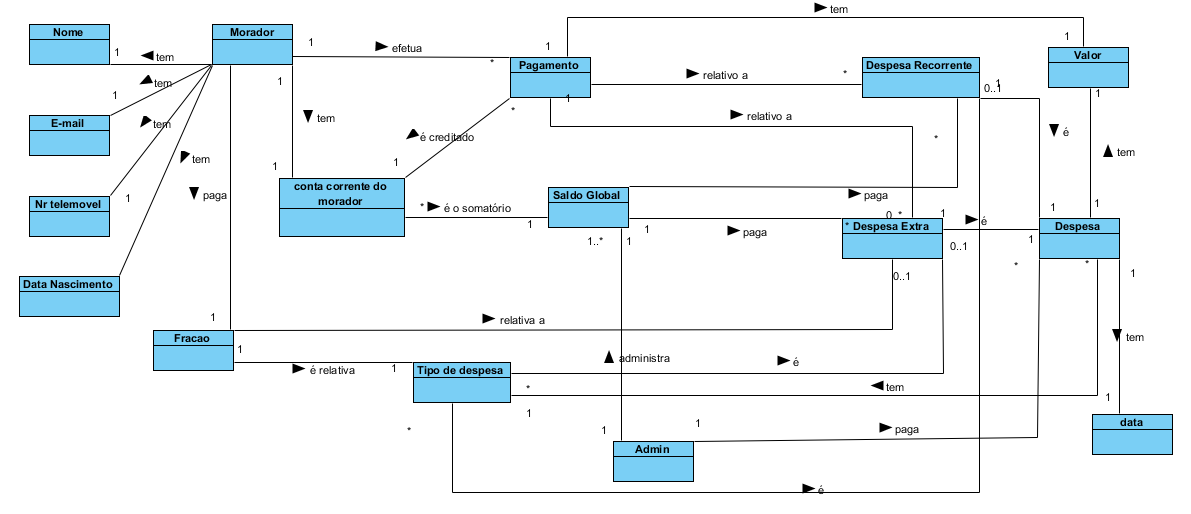
\includegraphics[scale=0.566]{modelodominio}  
	\caption{Modelo Dominio}  
\end{figure}


\section{Diagramas de Use Case}


\begin{figure}[htb!]
	\centering
	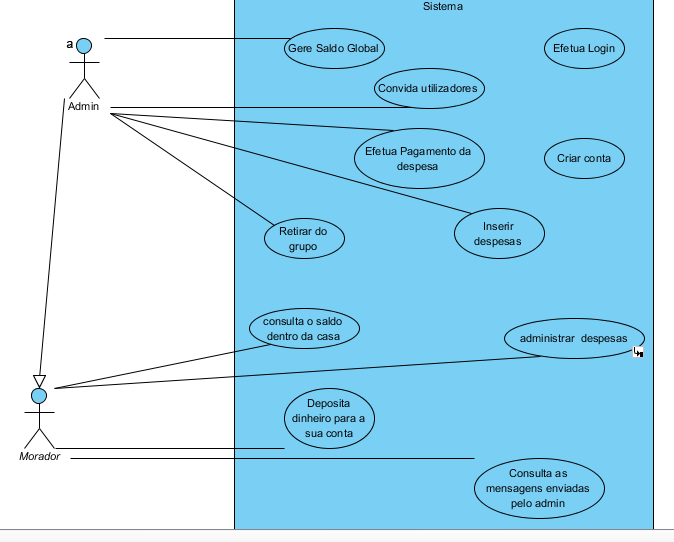
\includegraphics[scale=0.7]{usecase1}  
	\caption{Modelo Use Case}  
\end{figure}


\newpage
\section{Mockups}




